\section{Strain Analysis}
    \label{Sec:Results_Energy}
%! Motivation
The structural properties of the thin film, namely its mosaicity and lattice distortion depend crucially on the growth process.
It turned out that the absorption of energy at the laser entrance window alters the growth rate and the crystallinity much more dominantly than the growth temperature or the oxygen partial pressure (cf.\ \ref{Sec:Results_Preliminary}).
A similar effect was observed when targets were used for fabrication that exhibit a non-planar surface and tracks that were carved during previous ablations (cf.\ \ref{Sec:Results_Doping}).
Because the structural properties of the thin film also influence its electrical properties (cf.\ \ref{Sec:Results_Doping}), the following investigations focus on the origin of the observed variations in strain and \textomega-FWHM.
This is further motivated by the observation that a deliberate and controlled variation of laser spot size on the target surface yields a large reduction of \textomega-FWHM as well as a reduced shift of the peak position in the \thetaomega-pattern (Fig.\,\ref{Fig:Results_3_motivation}).
This was achieved by varying the lens position (cf.\ \ref{Fig:Methods_pld}) such that the laser spot size increases, yielding smaller fluence and larger ablation area on the target surface.
\begin{figure}[h]
    \centering
    \includegraphics{3_fluence_motivation.eps}
    \caption{
    \thetaomega-patterns for two \textit{c}-plane samples fabricated with different laser focus on the target.
    The inset displays the diffractograms of the corresponding \textomega-scans performed on the respective reflections.
    The ZnO-doped (low) target was used without a fixed $r_\mathrm{PLD}$ but with uniform ablation on the whole target surface.
    }
    \label{Fig:Results_3_motivation}
\end{figure}

\subsection{Experiment}
    %! Sample Fabrication
\subsubsection*{Sample Fabrication}
For all following depositions, the laser entrance window was cleaned before each process.
A pure \cro\ target was used for deposition of thin films on $5\times\qty{5}{\mm\squared}$ sapphire substrates in the four aforementioned orientations.
A first series of samples was produced by only varying the pulse number to achieve a series of thin films with varying thickness but constant laser fluence during deposition.
Therefore, the influence of thickness and growth rate can be deconvoluted.
% This is necessary, because the series of thicknesses that was achieved in the prior experiments was correlated to a series of growth rates.
The pulse energy was set to \qty{650}{\milli\joule} and the lens position to \qty{-2}{\cm}, resulting in a laser spot size of \qty{8}{\mm\squared}.
As described in section \ref{Sec:Methods_pld}, the laser pulse energy inside the PLD chamber is significantly lower than \qty{650}{\milli\joule}, due to passing a mask and absorption at the mirror, UV lens and laser entrance window.
By accounting for this attenuation, the resulting fluence on the PLD target is approx.\ \qty{2}{\joule\per\cm\squared}.
This corresponds to the standard configuration during all previous processes (\textcolor{magenta}{$\blacksquare$} in Fig.\,\ref{Fig:Methods_fluence}).
This was repeated for three other lens positions, namely \qtylist{0;1;2}{\cm}, resulting in lower fluences of \qtylist{1.1;0.8;0.6}{\J\per\cm\squared}, respectively.
In Fig.\,\ref{Fig:Methods_fluence}, the yellow circles represent those laser fluences.
This set of samples is referred to as the 1st batch and is listed in Tab.\,\ref{Tab:Results_3_batch1}.
The laser spot sizes for different lens positions are depicted in Fig.\,\ref{Fig:Results_3_laserSpotSize}.

\begin{figure}
    \centering
    \includegraphics{laserSpotSize}
    \caption{
        Laser spot size $A$ depending on the lens position $L$: measured data (black) and fit according to $A(L)=a_2L^2+a_1L+a_0$ (red dashed).
        The fit parameters $a_2$, $a_1$ and $a_0$ are \qty{0.74}{\mm\squared\per\cm\squared}, \qty{5.3}{\mm\squared\per\cm} and \qty{15.6}{\mm\squared}, respectively.
    }
    \label{Fig:Results_3_laserSpotSize}
\end{figure}
\begin{figure}
    \centering
    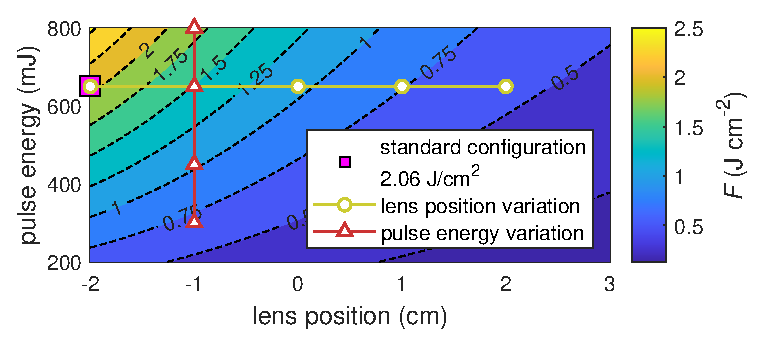
\includegraphics{fluence.eps}
    \caption{Laser energy density depending on the applied pulse energy and lens position. Smaller lens positions yield smaller spot sizes. A value of \qty{-2}{\cm} corresponds to the lens being as close as possible to the laser entrance window in the setup used for this work.
    The default configuration of \qty{650}{\milli\joule} and \qty{-2}{cm} yields typical fluences of about \qty{2}{\J\per\square\cm}.
    The triangles and circles represent the variation of laser fluence in this work, achieved by varying the pulse energy and lens position, respectively.}
    \label{Fig:Methods_fluence}
\end{figure}
\begin{table}
    \centering
    \caption{
        Processes of the first and second batch.
        For the first batch, a constant laser pulse energy of \qty{650}{\milli\J} was applied.
        The second batch was obtained by fixing the laser spot size to \qty{10}{\mm\squared}.
        For every process, \cro\ was deposited on four sapphire substrates with different orientations of \textit{c}-, \textit{r}-, \textit{m}- and \textit{a}-plane.
    }
    \begin{tabular}{lSSSSSS}
        \toprule
        
        & {$L$ (\unit{\cm})}
        & {$E_\mathrm{L}$ (\unit{\milli\J})}
        & {$A$ (\unit{\mm\squared})}
        & {$F$ (\unit{\J\per\cm\squared})}
        & {pulses (1k)}
        & {$t$ (\unit{\nm})}\\
        \midrule
        \parbox[t]{3mm}{\multirow{11}{*}{\rotatebox[origin=c]{90}{Batch 1}}}
        &-2      &  650      &   8       &   2.1       &   5       &   25  \\
        &        &           &           &           &   10      &   45  \\
        &        &           &           &           &   20      &   80  \\
        &        &           &           &           &   40      &   170  \\
        &        &           &           &           &   70      &   210  \\ \cmidrule{2-7}
        &0       &           &   16      &   1.1       &   8       &   40  \\
        &        &           &           &           &   20      &   90  \\
        &        &           &           &           &   35      &   40  \\ \cmidrule{2-7}
        &1       &           &   22      &   0.8     &   20      &   50  \\
        &        &           &           &           &   40      &   65  \\ \cmidrule{2-7}
        &2       &           &   29      &   0.6     &   17      &   30
        \\
        \midrule
        \parbox[t]{3mm}{\multirow{6}{*}{\rotatebox[origin=c]{90}{Batch 2}}}
        &-1      &  300      &   10       &   0.7       &   40       &   90  \\
        &        &  300      &            &   0.7       &   70       &   150  \\ \cmidrule{3-7}
        &        &  450      &            &   1.0       &   40       &   150  \\
        &        &  450      &            &   1.0       &   50       &   150  \\ \cmidrule{3-7}
        &        &  650      &            &   1.5       &   40       &   200  \\ \cmidrule{3-7}
        &        &  800      &            &   1.8       &   35       &   170  \\
        \bottomrule


    \end{tabular}
    \label{Tab:Results_3_batch1}
\end{table}

To investigate the influence of fluence independent of ablation area, a 2nd batch of samples was fabricated with a laser spot size of aprox.\ \qty{10}{\mm\squared} ($L=\qty{-1}{\cm}$) but varying laser pulse energy:
\qtylist{300;450;650;800}{\milli\joule}.
The achieved fluences are \qtylist{0.7;1.0;1.5;1.8}{\J\per\cm\squared} (red triangles in Fig.\,\ref{Fig:Methods_fluence}).
The pulse number was adjusted to achieve approximately the same thickness for all samples even though the growth rate vastly differs.
But note that for the different samples, the thickness is distributed from \qtyrange{100}{200}{\nm}.
Better results could be achieved in future experiments by first calibrating the growth rates for different fluences, and then adjusting the pulse numbers accordingly.
The process parameters of those samples are listed in Tab.\,\ref{Tab:Results_3_batch1}.

%! Measurements
\subsubsection*{Measurements}
For all samples, \thetaomega-scans as well as \textomega-scans were performed.
The symmetric reflections probed by the latter were (00.6), (02.4), (30.0) and (22.0) for \textit{c}-, \textit{r}-, \textit{m}- and \textit{a}-plane, respectively.
For \textit{r}- and \textit{a}-plane samples, the higher order reflection was chosen because the distance between the \cro\ peak and the \alo\ peak caused by \ce{W}-L\textalpha\textsubscript{1} radiation increases with higher angles.
Because both peaks are located at similar angles, this approach reduces the contribution of the substrate to the thin film Rocking curves.
% The thickness of all samples was determined by spectroscopic ellipsometry measurements.
To obtain more information about the relation between in-plane and out-of-plane lattice constants, \glspl{RSM} were performed on selected samples.
For every orientation, lattice planes have been chosen that have both a rather small tilt and high intensity:

\paragraph{\textit{c}-plane}
    For \textit{c}-plane samples, the thickness series grown at $L=\qty{-2}{\cm}$ and therefore a laser spot size of \qty{8}{\mm\squared} ($F=\qty{2.1}{\J\per\cm\squared}$) of the 1st batch was investigated.
    The asymmetric reflection that was used for probing the relaxation process is (02.10), which has an inclination angle of approx.\ \qty{32}{\degree} with respect to the sample surface.
\paragraph{\textit{r}-plane}
    All \textit{r}-plane samples fabricated in the 2nd batch with different laser pulse energies were investigated with \glspl{RSM}.
    For each sample, the $x$-axis of the sample -- containing the projection of the \textit{c}-axis -- is found by performing a \textphi-scan on the (03.0) reflection:
    This set of lattice planes has an inclination with respect to the surface, so the position of the peak in the diffraction pattern of the \textphi-scan reveals the $x$-axis.
    In this azimuth, an \gls{RSM} is recorded around the asymmetric (03.0) reflection and the symmetric (02.4) reflection.
    By rotating $\Delta\phi=\qty{90}{\degree}$, the $y$-axis lays in the scattering plane and another \gls{RSM} is performed around the symmetric (02.4) reflection.
    The twofold measurement of the symmetric reflection is necessary to calculate a possible lattice plane tilt for both $x$- and $y$-direction.
    % Note that no shear is calculated due to the asymmetric nature of the (03.0) reflection with respect to the \textit{r}-orientation\footnote{
        % For \textit{m}- and \textit{a}-plane rhombohedral structures, the crystal is symmetric under the transformation $\phi\rightarrow\phi+\qty{180}{\degree}$, which is not the case for \textit{r}-plane.
    % }.
    After performing the various corrections described in section \ref{Sec:Methods_RSM}, the tilt angles can be calculated for both azimuths by
    \begin{eqnarray}
        \theta = \arccos\left(
            \frac{q_\perp}{|\mathbf{q}|}
        \right) \cdot\mathrm{sgn}\left(q_\parallel\right)\,,
        \label{Equ:Results_3_tiltAngle}
    \end{eqnarray}
    with $q_\perp$ and $q_\parallel$ being the \gls{oop}\ and \gls{ip}\ components of the scattering vector $\mathbf{q}$, respectively.
    The \gls{ip}\ and \gls{oop}\ strains are determined by comparing the observed (03.0) scattering vector to the scattering vector calculated from \cro\ bulk lattice constants:
    \begin{equation}
        \mathbf{q}_\mathrm{(03.0)} = 
        \left|\mathbf{q}_\mathrm{(03.0)}\right|\cdot
        \begin{pmatrix}
            \cos\alpha_{(03.0)|r}\\
            \sin\alpha_{(03.0)|r}
        \end{pmatrix}\,,
    \end{equation}
    with $|\mathbf{q}_{(03.0)}|$ calculated from \eqref{Equ:Methods_qAbs} and \eqref{Equ:Methods_dhkl}.
    $\alpha_{(03.0)|r}$ denotes the angle between the (03.0) reflection and the normal of the \textit{r}-planes; it can be calculated from \eqref{Equ:Methods_angleWRTc}:
    \begin{equation}
        \alpha_{(03.0)|r}
        = \qty{90}{\degree}-\left(
            \alpha_{(03.0)|c}-\alpha_{(01.2)|c}
        \right)
        = \alpha_{(01.2)|c}
        = \qty{57.62}{\degree}\,.
    \end{equation}
\paragraph{\textit{m}-plane}
    Similar to the \textit{r}-plane samples, all \textit{m}-plane samples from the 2nd batch were investigated.
    The samples were aligned to the $x$-axis by performing a \textphi-scan on the asymmetric (30.6) reflection, and an \gls{RSM} was recorded afterwards.
    By rotating $\Delta\phi=\qty{180}{\degree}$ while maintaining $2\theta$ and $\omega$, the scattering condition for $(30.\overline{6})$ is probed and an \gls{RSM} was recorded.
    The symmetric reflection (30.0) was also measured in this azimuth.
    The tilt angle and shear angle can be calculated according to \eqref{Equ:Results_3_tiltAngle} and \eqref{Equ:Methods_shearAngle}, respectively.
    As described in further detail in appendix \ref{Sec:App_Calc_mPlane}, the lattice constants can be calculated from the components of the scattering vectors:
    \begin{align}
        a_\perp &= \frac{\sqrt{12}}{q_\perp^{(30.\pm6)}} \,,\\
        a_\perp &= \frac{\sqrt{12}}{q_\perp^{(03.0)}}\,,\\
        c &= \frac{6}{q_\parallel^{(30.\pm6)}} \,.
    \end{align}
    $a_\perp$ denotes the $a$ lattice constant in direction of the normal to the sample surface.
    By rotating $\Delta\phi=\qty{90}{\degree}$, the \textit{y}-axis can be probed via asymmetric reflections $(\overline{4}2.0)$ and (22.0), which differ in the azimuth by $\Delta\phi=\qty{180}{\degree}$.
    A second symmetric reflection (30.0) is recorded in this azimuth.
    Similar to the $x$-axis, the tilt and shear angles, as well as the lattice constants can be calculated:
    \begin{align}
        (4\overline{2}.0):&\quad
            a_\perp = \frac{\sqrt{12}}{q_\perp^{(4\overline{2}.0)}}
            \quad,\quad
            a_\parallel = \frac{2}{q_\parallel^{(4\overline{2}.0)}}\,,\\
        (22.0):&\quad
            a_\perp = \frac{\sqrt{12}}{q_\perp^{(22.0)}}
            \quad,\quad
            a_\parallel = \frac{2}{q_\parallel^{(22.0)}}\,,\\
        (30.0):&\quad
            a_\perp = \frac{\sqrt{12}}{q_\perp^{(03.0)}}\,.
    \end{align}
    $a_\parallel$ denotes the $a$ lattice constant parallel to the $y$-axis.
    For detailed calculations of the former equations, see appendix \ref{Sec:App_Calc_mPlane}.
    Note that all 6 measured reflections yield a value for $a_\perp$, and 2 measured reflections each yield 2 values for $c$ and $a_\parallel$, respectively.
    Therefore, for each lattice constant, the mean value is evaluated and the error is estimated by the standard deviation (cf.\ Fig.\,\ref{Fig:Results_3_pulse_ma_strainTilt}a).
\paragraph{\textit{a}-plane}
    All \textit{a}-plane samples from the 2nd batch were investigated and the method is similar to the one applied to the \textit{m}-plane samples.
    The azimuth of the \textit{x}-axis is found by performing a \textphi-scan on the (22.6) reflection, which also served for an \gls{RSM}.
    Rotating by $\Delta\phi=\qty{180}{\degree}$ yields the $(22.\overline{6})$ reflection and (22.0) is also measured.
    Similar to above, the sample is rotated by \qty{90}{\degree} to align to the $y$-axis and two more asymmetric reflections are recorded: (30.0) and (03.0).
    A second \gls{RSM} of (22.0) is also performed.
    This yields the following lattice constants for the $x$-axis:
    \begin{align}
        a_\perp &= \frac{4}{q_\perp^{(22.\pm6)}} \,,\\
        a_\perp &= \frac{4}{q_\perp^{(22.0)}}\,,\\
        c &= \frac{6}{q_\parallel^{(22.\pm6)}} \,,
    \end{align}
    and for the $y$-axis:
    \begin{align}
        (30.0):&\quad
            a_\perp = \frac{3}{q_\perp^{(30.0)}}
            \quad,\quad
            a_\parallel = \frac{3}{\sqrt{3}q_\parallel^{(30.0)}}\,,\\
        (03.0):&\quad
            a_\perp = \frac{3}{q_\perp^{(03.0)}}
            \quad,\quad
            a_\parallel = \frac{3}{\sqrt{3}q_\parallel^{(03.0)}}\,,\\
        (22.0):&\quad
            a_\perp = \frac{4}{q_\perp^{(22.0)}}\,.
    \end{align}
    For detailed calculations, see appendix \ref{Sec:App_Calc_aPlane}.
    Again, for the lattice constants obtained from several reflections, the mean and standard deviation are calculated (cf.\ Fig.\,\ref{Fig:Results_3_pulse_ma_strainTilt}b).

    \label{Sec:Results_3_Experiment}
\subsection{Results}
    % The analysis of the data will be structured into the analysis of (i) \textit{c}-plane, (ii) \textit{r}-plane and (iii) \textit{m}- and \textit{a}-plane samples.
% In the following, some general remarks on the fabricated samples will be made.

%* lens pos series
In Fig.\,\ref{Fig:Results_3_lensGrowthRate}, a detailed view into the growth rates of the samples of the 1st batch is given.
First of all, for a fixed fluence (false color), increasing the pulse number decreases the growth rate.
This is expected, because the coating of the laser entrance window increases during the process.
By fixing a pulse number to \qty{20000}{pulses}, an increase in growth rate is observed for a regime of decreasing fluence from \qtyrange{2}{1}{\joule\per\cm\squared} (Fig.\,\ref{Fig:Results_3_lensGrowthRate} bottom).
This can be explained by the fact that the reduction of fluence is due to increasing laser spot size.
When the fluence is still above the ablation threshold for the target material, an increasing ablation area results in an increasing growth rate.
But at some point, the fluence is too low to ablate the material and then the growth rate decreases, even though the ablation area increases.
This can be observed at around \qty{1.2}{\joule\per\cm\squared} in Fig.\,\ref{Fig:Results_3_lensGrowthRate}, which is therefore an estimate for the ablation threshold.
\begin{figure}
    \centering
    \includegraphics{3_lensPos_growthrates.pdf}
    \caption{
    Growth rates of the samples from the 1st batch, i.e.\ samples with different laser spot size and therefore different laser fluence (false color), as well as different pulse number each (cf.\ Tab.\,\ref{Tab:Results_3_batch1}).
    The growth rate is visualized as depending on the pulse number (top) and depending on the laser fluence on the target for a fixed pulse number of \qty{20000}{} (bottom).
    The data points are the mean of the four samples with \textit{c}-, \textit{r}-, \textit{m}- and \textit{a}-orientation, that were obtained from every process.
    The errorbar displays the standard deviation.
s    }
    \label{Fig:Results_3_lensGrowthRate}
\end{figure}
%
%* Pulse energy series
For the growth rates of the samples of the 2nd batch (Fig.\,\ref{Fig:Results_3_pulseGrowthRate}), a similar conclusion can be drawn.
Reducing the fluence via decreasing laser pulse energy below approx.\ \qty{1.5}{\joule\per\cm\squared} results in a decrease of growthrate from \qtyrange{5}{2}{\pm\per\pulse}.
The ablation threshold can be localized between \qtylist{1;1.5}{\joule\per\cm\squared}, which is in accordance to the value obtained for the 1st batch.
\begin{figure}
    \centering
    \includegraphics{3_pulseEnergy_growthrates.eps}
    \caption{Growth rates of samples from the 2nd batch, i.e.\ samples with different laser pulse energy, but same laser spot size on the target, depending on laser fluence on the target surface.
    The data points are the mean of thicknesses of the four orientations, similar to Fig.\,\ref{Fig:Results_3_lensGrowthRate}.}
    \label{Fig:Results_3_pulseGrowthRate}
\end{figure}
        \subsubsection{\textit{c}-plane: Laser Spot Size Variation}
            %! theta omega
The \gls{oop}\ strain calculated via \eqref{Equ:Results_oop_strain_def} for all samples of the 1st batch is displayed in Fig.\,\ref{Fig:Results_3_lensStrain}.
Consider the \textit{c}-plane oriented samples of the 1st batch that had a fixed lens position yielding a fluence of approx.\ \qty{2}{\joule\per\cm\squared}, but varying thickness (brown squares in Fig.\,\ref{Fig:Results_3_lensStrain}).
A clear dependence of the \gls{oop}\ strain can be observed: thinner samples yield higher strain.
The layers become relaxed for thicknesses above approx.\ \qty{170}{\nm}.
For low thicknesses, the strain approaches the predicted value for pseudomorphic growth of \cro\ on \ce{Al2O3}, which is \qty{3.90}{\percent} (cf.\ Tab.\,\ref{tab:d_strained}).
\begin{figure}
    \centering
    \includegraphics{3_lensPos_strain.eps}
    \caption{
        Out-of-plane strain calculated from \thetaomega-patterns for all samples from the 1st batch, depending on thickness and laser fluence (false color).
    }
    \label{Fig:Results_3_lensStrain}
\end{figure}
%! RSMs strain
The recorded \glspl{RSM} of the (02.10) reflection can confirm that this observation of \gls{oop}\ strain is due to pseudomorphic growth.
In Fig.\,\ref{Fig:Results_3_cRSMs}, one can observe a shift of $q_\parallel^{(02.10)}$ to higher values for lower thicknesses.
This corresponds to a decrease of the \gls{ip}\ lattice constant, which is the expected behavior for pseudomorphic growth, because the \gls{ip}\ $a$ lattice constant of \textit{c}-oriented \ce{Al2O3} is \qty{0.2}{\angstrom} smaller than for \cro\ (cf.~Tab.\,\ref{Tab:sesquiLatticeConstants}).
The tensile \gls{oop}\ strain observed via \thetaomega-scans can also be confirmed by the fact that the \gls{oop}\ component $q_\perp^{(02.10)}$ is decreasing for thinner samples.
The reduction of signal intensity is attributed to the thickness, but could also be a result of decreasing crystal quality (cf.~Fig.\,\ref{Fig:Results_3_lensOmega}).
\begin{figure}
    \centering
    \includegraphics{3_lensPos_RSM_c.png}
    \caption{
        \glspl{RSM} of the (02.10) reflection for \textit{c}-plane oriented samples with varying thickness.
        The laser spot size was \qty{8}{\mm\squared}, resulting in a fluence of approx.\ \qty{2}{\J\per\cm\squared}.
        The reflection in the upper right corner corresponds to the (02.10) reflection of the sapphire substrate.
    }
    \label{Fig:Results_3_cRSMs}
\end{figure}
When looking into the remaining samples that were fabricated with larger laser spot sizes but similar thickness of \qty{50}{\nm} (bluish squares in Fig.\,\ref{Fig:Results_3_lensStrain}), it becomes clear that the \gls{oop} strain is also slightly reduced for lower fluences.
But note that this effect is less dominant when compared to the influence of thickness.

%! omega
In Fig.\,\ref{Fig:Results_3_lensOmega}, the \textomega-FWHM is depicted in dependence on the film thickness and laser fluence for the 1st batch.
As before, consider the samples with smallest laser spot size (largest fluence) first:
increasing the thickness is clearly correlated to a decreasing \textomega-FWHM.
Therefore, thicker samples yield \emph{both} less strained and more crystalline films.
This is an unexpected result, because as shown in section \ref{Sec:Theory_Relaxed}, relaxation is mediated by dislocations which should worsen the crystal quality.
Note that there is an outlier to this behavior for the sample with a thickness of approx.\ \qty{30}{\nm}.
When considering the \textomega-pattern of this sample (Fig.\,\ref{Fig:App_3_cOmegaOutlier}a), it becomes clear that the non-\textsc{Voigt} shape makes the determination of \gls{FWHM} difficult.
Therefore, not too much attention should be paid to this data point.
When considering the samples fabricated with lower fluences (bluish squares in Fig.\,\ref{Fig:Results_3_lensOmega}), a much more dominant influence of laser spot size on the crystallinity can be observed.
\begin{figure}
    \centering
    \includegraphics{3_lensPos_omega.eps}
    \caption{
        \textomega-FWHM for all samples from the 1st batch, depending on thickness and laser fluence (false color).
        The corresponding diffractograms are depicted in Fig.\,\ref{Fig:App_3_lens_omega}.
    }
    \label{Fig:Results_3_lensOmega}
\end{figure}
%! correlation
This can be summarized by stating that the thickness of the samples is the dominant influence on the \gls{oop}\ strain, because the thickest samplest yielded less strain than the thinner samples with lowest fluence (Fig.\,\ref{Fig:Results_3_lensStrain}).
However, for the \textomega-FWHM, the reverse is observed, namely that even the thickest samples (which exhibit better quality than thinner samples of the same lens position) have a much higher \textomega-FWHM when compared to thinner samples fabricated with less fluence.
This can be seen in Fig.\,\ref{Fig:Results_3_lensCorrelation}, where the \textomega-FWHM is visualized depending on the \gls{oop}\ strain of the corresponding sample:
A linear behavior (correlation) is observed for each set fluence; but there are two different regimes in total, with the high-fluence regime generally showing higher \textomega-FWHM.
        \subsubsection{\textit{c}-plane: Pulse Energy Variation}
            %! Theta Omega
The \gls{oop}\ strain for the \textit{c}-plane oriented samples fabricated with various laser pulse energies, but constant laser spot size, is depicted in Fig.\,\ref{Fig:Results_3_pulseStrain}.
Note that there is still a distribution of thickness from \qtyrange{100}{200}{\nm}, even though it was tried to counteract this by adjusting the pulse numbers.
Therefore, the thickness is also displayed via false color to account for the convolution of thickness with laser fluence.
The strain is overall smaller ($<\qty{2}{\percent}$) than for the 1st batch, because the 2nd batch contained samples with thickness $t>\qty{100}{\nm}$ which yields smaller strains as seen before.
No systematic dependence on the laser fluence is observed, which may be explained by the still remaining thickness distribution which overlaps the fluence variation.
This effect could be strong enough to overshadow the impact of laser pulse energy, as it was shown in the previous experiments that the thickness is the dominant factor for the \gls{oop}\ strain.
For example, note the sample fabricated with $F=\qty{1.5}{\J\per\cm\squared}$ (\textcolor{col-darkGreen}{$\blacksquare$} in Fig.\,\ref{Fig:Results_3_pulseStrain}), which exhibits the lowest strain, even though having higher fluence value than other samples.
This can be explained by the fact that with $t=\qty{200}{\nm}$, it is the thickest sample of the batch and therefore the lowest strain is expected (cf.\ Fig.\,\ref{Fig:Results_3_lensStrain}).
\begin{figure}
    \centering
    \includegraphics{3_pulseEnergy_strain.eps}
    \caption{
        Out-of-plane strain calculated from \thetaomega-patterns for all samples from the 2nd batch (varying laser pulse energy), depending on laser fluence and thickness (false color).
    }
    \label{Fig:Results_3_pulseStrain}
\end{figure}

%! Omega
In Fig.\,\ref{Fig:Results_3_pulseOmega}, the \textomega-FWHM is depicted depending on the laser fluence and film thickness for the 2nd batch.
The previously observed relation is confirmed: increasing fluences result in higher \textomega-FWHMs.
Namely, reducing the fluence by a factor of 2 results in a crystal quality improvement by one order of magnitude.
Note that for a fluence of approx.\ \qty{1}{\J\per\cm\squared}, two samples \texttt{A} and \texttt{B} with same thickness of \qty{150}{\nm} exhibit very different \textomega-FWHM of $\Delta\omega_\mathtt{A}=\qty{8}{\arcminute}$ and $\Delta\omega_\mathtt{B}=\qty{49}{\arcminute}$.
The \textomega-patterns are depicted in Fig.\,\ref{Fig:App_3_cOmegaOutlier}b.
Note that both diffractograms have \textsc{Voigt} shape, so the discrepancy may not be attributed to the determination of the \gls{FWHM}.
On the contrary, note that for the whole process \texttt{B}, which represents a set of samples with \textit{c}-, \textit{r}-, \textit{m}- and \textit{a}-orientation, a determination of FWHM was possible only for the \textit{c}-plane samples\footnote{
    This is why in Fig.\,\ref{Fig:Results_3_pulseOmega}, only the upper left \textit{c}-plane tile has two data points at $F\approx\qty{1}{\J\per\cm\squared}$.
}.
In Fig.\,\ref{Fig:App_3_w6930}, the \textomega-patterns of samples of all orientations from this process are depicted.
The non-\textsc{Voigt} shape for the orientations other than \textit{c}-plane as well as the unexpectedly high \textomega-FWHM for \textit{c}-plane sample indicate that the process yielded samples with poor crystal quality.
The origin of this observation is not entirely clear, but since both \texttt{A} and \texttt{B} were conducted with the same process parameters with similar growthrate of $g_\mathtt{A}=\qty{3}{\pm\per\pulse}$ and $g_\mathtt{B}=\qty{3.75}{\pm\per\pulse}$, an unknown effect must have influenced the thin film deposition substantially.
% \sout{something irregular must have been occured during the process}.

\begin{figure}
    \centering
    \includegraphics{3_pulseEnergy_omega.eps}
    \caption{
        \textomega-FWHM for all samples from the 2nd batch (varying laser pulse energy), depending on laser fluence and thickness (false color).
        The corresponding diffractograms are depicted in Fig.\,\ref{Fig:App_3_pulse_omega}. 
    }
    \label{Fig:Results_3_pulseOmega}
\end{figure}
        \subsubsection{\textit{r}-plane: Laser Spot Size Variation}
            In Fig.\,\ref{Fig:Results_3_lensStrain}, the \gls{oop}\ strain for the \textit{r}-plane samples fabricated with varying laser spot size is shown.
The overall strain is with less than \qty{1}{\percent} lower when compared to the \textit{c}-plane samples, exhibiting values up to \qty{4}{\percent} for thin samples.
In particular, the predicted value for \gls{oop}\ strain during pseudomorphic growth of \cro\ on \ce{Al2O3} of \qty{2.41}{\percent} is not reached (cf.\ Tab.\,\ref{tab:d_strained}).
As can be seen in a detailed view (Fig.\,\ref{Fig:App_3_lensStrain_zoomed}), the strain depends on the thickness:
it decreases from \qty{0.8}{\percent} to \qty{0.5}{\percent} for an increment of thickness from \qty{50}{\nm} to \qty{200}{\nm}.
This is in accordance to the bahavior observed for the \textit{c}-plane samples, albeit less pronounced.
Furthermore, for a fixed thickness, decreasing the fluence also results in less strained thin films, which is similar to the behavior of the \textit{c}-plane samples.
The \textomega-FWHM obtained from the (02.4) reflection is depicted in Fig.\,\ref{Fig:Results_3_lensOmega}.
Similar to the \textit{c}-plane samples -- but less pronounced--, increasing the thickness results in less mosaicity, which is also achieved by reducing the fluence.
Note that the overall \textomega-FWHM is between \qtylist{50;90}{\arcminute} which differs for the \textit{c}-plane samples, where a lower fluence yielded samples with $\Delta\omega<\qty{10}{\arcminute}$ (cf. Fig.\,\ref{Fig:Results_3_lensOmega}).
Therefore, increasing the thickness and reducing the fluence by varying laser spot position may increase the crystal quality, but not to an amount comparable to \textit{c}-plane oriented thin films.

        \subsubsection{\textit{r}-plane: Pulse Energy Variation}
            %! thetaomega strain
In Fig.\,\ref{Fig:Results_3_pulseStrain}, the \gls{oop}\ strain is depicted for varying laser pulse energies (2nd batch).
Independent of thickness, the fluence determines the strain of the thin films.
The overall strain is below \qty{0.4}{\percent}, and thereby comparable to the samples obtained from processes in the 1st batch with larger laser spot sizes.
%! RSM: strain
\begin{figure}
    \centering
    \includegraphics{3_pulseEnergy_completeStrain_r.eps}
    \caption{
        In-plane and out-of-plane strain for the \textit{r}-plane samples from the 2nd batch, calculated from the peak positions of the \glspl{RSM} described in~\ref{Sec:Results_3_Experiment} (left).
        Tilt along the $x$-axis (purple ordinate) and $y$-axis (blue ordinate), determined from symmetric reflections (right).
        Note the different scaling of the ordinates, indicating less tilt along the $y$-axis.
    }
    \label{Fig:Results_3_pulse_r_StrainTilt}
\end{figure}
A detailed view on the strain for those samples is given in Fig.\,\ref{Fig:Results_3_pulse_r_StrainTilt} which is based on the evaluation of \glspl{RSM} that were performed as described in~\ref{Sec:Results_3_Experiment}.
The \gls{oop}\ strain was calculated from both asymmetric (green triangle) and symmetric (yellow squares) reflections.
The latter is equivalent to the calculation from the peak position in \thetaomega\ diffraction patterns.
It can be observed that the increasing tensile \gls{oop}\ strain comes along with an increasing \gls{ip}\ compressive strain, ranging from \qty{-0.2}{\percent} to \qty{-0.8}{\percent}.
Therefore, the \gls{oop} strain may be attributed to a partial pseudomorphic growth mode, because the \ce{Al2O3} lattice constants are smaller than the ones for \cro.
The compressive strain is then due to an aligning of in-plane lattice constants.

Note that the values for \gls{oop}\ strain obtained from \thetaomega-scans (cf.\ Fig.\,\ref{Fig:Results_3_pulseStrain}) are only qualitatively confirmed:
the strain measured from the symmetric \gls{RSM} is approx.\ 0.2 percentage points below the value obtained from \thetaomega-scans.
A comparison of both methods is given in Fig.\,\ref{Fig:Results_3_r_strainDiscrepancy}, where both a \thetaomega\ pattern and a symmetric \acrshort{RSM} of the are depicted for one sample ($F=\qty{1.1}{\J\per\cm\squared}$), as well as the calculated strain for all samples with different laser pulse energy.
\begin{figure}[ht]
    \centering
    \includegraphics{3_misc_pulse_r_discrepancy.png}
    \caption{
        Out-of-plane strain for the \textit{r}-plane samples fabricated with varying laser pulse energy (right).
        For the sample with $F=\qty{1.1}{\J\per\cm\squared}$, the \thetaomega\ pattern (top left) and \gls{RSM} (bottom left) are depicted.
        The black diamond ($\blacklozenge$) marks the position of the (02.4) reflection in the 1D \thetaomega\ pattern and 2D \gls{RSM}.
    }
    \label{Fig:Results_3_r_strainDiscrepancy}
\end{figure}
The origin of this discrepancy may lie in on of the corrections that was applied the \glspl{RSM}, but not to the \thetaomega\ patterns.
However, the correction of the substrate peak position in 2D reciprocal space (rotation and stretching, cf.\ section \ref{Sec:Methods_RSM}) corresponds to a shift of the whole 1D \thetaomega\ pattern to match the substrate peak.
The latter was done for the evaluation of \thetaomega-scans on which Fig.\,\ref{Fig:Results_3_pulseStrain} is based.
But the correction of thin film tilt which is done for \glspl{RSM} was not done for the \thetaomega-scans.
This can be seen in Fig.\,\ref{Fig:Results_3_r_strainDiscrepancy}, where the \thetaomega\ pattern corresponds to a line with $q_\parallel=\mathrm{const.}=0$ in the reciprocal space.
The peak on this line has the same $q_\perp$ coordinate as the RSM peak not corrected to thin film tilt (both visualized as black diamonds, $\blacklozenge$).
But if the (03.0) peak is rotated by the value of thin film tilt (counterclockwise), the $q_\perp$ component slightly increases.
Therefore it follows that
$$q_\perp^\mathrm{RSM, corrected}
>q_\perp^\mathrm{RSM, uncorrected}
=q_\perp^{2\theta\mathrm{-}\omega}\,,$$
which results in a smaller \gls{oop}\ lattice constant obtained from RSMs.
Therefore, the \gls{oop}\ strain is smaller, when determined from symmetric RSMs.
Note that a \textomega-optimization prior to a \thetaomega-scan is done for correcting a tilt of the \textit{substrate}, which is different from the correction of thin film tilt.

But even though this is a significant difference in evaluation between \thetaomega-patterns and \glspl{RSM}, the discrepancy between both methods does not change significantly when the thin film tilt decreases from \qty{40}{\arcminute} to \qty{10}{\arcminute}.
So further analysis has to be done for the applied evaluation methods.
In general it has to be noted that the precision of the \gls{oop}\ strain obtained from \glspl{RSM} depends on (i) the peak position of the reflection, (ii) the peak position of the corresponding substrate peak (for substrate correction) and (iii) the peak position of the asymmetric peaks (for shear correction, not done for \textit{r}-plane).
These values are subject to a certain amount of uncertainity, which results in an ill-defined error.
% Those positions were not obtained by fitting a 2D \textsc{Voigt} profile to the \glspl{RSM}, but by reading the peak position \enquote{by hand}.
% This may result in an undefined error.

{\sloppy % fix problems with the word "squares"
Another observation is that the \gls{oop}\ strain obtained from symmetric (yellow squares) and asymmetric reflections (green triangles) aligns for the two samples fabricated with higher fluences only (cf.\ Fig.\,\ref{Fig:Results_3_pulse_r_StrainTilt}).
The discrepancy observed for the lower fluences is unexpected.
In Fig.\,\ref{Fig:Res_3_RSMs_r}, all symmetric and asymmetric RSMs are displayed.
For the samples fabricated with \qtylist{650;800}{\milli\J}, accounting for the thin film tilt will result in a counterclockwise rotation of the reciprocal space.
Therefore, the observed (03.0) reflection (\textcolor{red}{$\blacksquare$}) has a smaller $q_\perp$ component compared to the predicted ($\blacklozenge$) peak position (after rotation).
This results in tensile (positive) strain -- which is in accordance with the values obtained from both symmetric RSM reflections and \thetaomega\ patterns.
For the samples with \qtylist{300;450}{\milli\J}, however, the thin film tilt is sufficiently small to result in compressive (negative) strain, i.e.\ the rotation of reciprocal space does not result in a smaller out-of-plane component $q_\perp$ of the thin film (\textcolor{red}{$\blacksquare$}) compared to the bulk value ($\blacklozenge$).

and is probably due to an error in evaluation of the \glspl{RSM}.
This is supported by the fact that for those two data points, the strain obtained from asymmetric reflections is almost exactly mirroring the value obtained from the symmetric reflections.
% This also confirms the previously stated hypothesis that the evaluation of either \gls{RSM} or \thetaomega-pattern exhibits a systematic error.
\par}
\begin{figure}
    \centering
    \includegraphics{3_misc_r_RSMs.png}
    \caption{
        Reciprocal space maps of four \textit{r}-plane oriented thin films fabricated with different laser pulse energy.
        The probed reflections are symmetric (02.4) (left) and asymmetric (30.0) (right).
        The peak with larger $q_\perp$ component corresponds to the substrate.
        For the RSMs of the asymmetric reflections, the expected peak position ($\blacklozenge$) as well as the observed peak positions (\textcolor{red}{$\blacksquare$}) are indicated.
        Note that the RSMs are already corrected such that the substrate peak aligns with the expected position.
        A thin film tilt is indicated by the nonzero in-plane component of the symmetric (02.4) reflection.
        For determination of thin film lattice constants, the RSM is rotated by the observed thin film tilt, which is not visualized in these images.
    }
    \label{Fig:Res_3_RSMs_r}
\end{figure}

%! RSM: tilt
As predicted by \textcite{grundmann2020b}, partially relaxed \textit{r}-plane thin films should exhibit a tilt of the thin film with respect to the substrate.
This tilt is indeed observed along the $x$-axis for all values of fluence, ranging from approx.\ \qty{10}{\arcminute} to \qty{40}{\arcminute} (purple triangles in Fig.\,\ref{Fig:Results_3_pulse_r_StrainTilt}).
A corresponding tilt along the $y$-axis is not observed: there, the tilt angles are two orders of magnitude lower and below \qty{0.4}{\arcminute}.
This is in agreement with elasticity theory which predicts a tilt only along the $x$-axis, because the prismatic slip systems responsible for relaxation along the $y$-axis yield tilt components of the \gls{bv} that cancel out on average (cf.\ section \ref{Sec:Theory_Relaxed}).
But note that the thin film tilt increases for higher fluences, which also results in a higher \gls{oop}\ strain.
This observation is unexpected, because the thin film tilt is a result of \emph{relaxation}, whereas strain is a result of partial \emph{pseudomorphic} growth.
So according to strain, higher fluences result in less relaxed layers -- according to tilt, higher fluences result in more relaxed layers.
This result indicates that an interplay of both processes is present and that for growth modes that exhibit no partially relaxed behavior, more sophisticated models for the relaxation mechanism must be applied.

%! omega
The \textomega-FWHM of the \textit{r}-plane samples of the 2nd batch is approx.\ \qty{50}{\arcminute} and has no significant dependence on both fluence or thickness (Fig.\,\ref{Fig:Results_3_pulseOmega}).
This confirms the previously obtained result for the samples fabricated with varying laser spot sizes.